\chapter{Geometry}
\label{sec:geom}
This section describes the variables and methods used to parameterize
the substructure geometry in \textit{FloatingSE}.  Typically,
substructure designs have fallen into three classical regimes, which are
shown in Figure \ref{fig:archetype}, each of which attains stability
through different physical mechanisms.  A spar derives its stability from a
deep drafted ballast.  A semisubmersible derives its stability from
distributed waterplane area, achieved with offset columns spread evenly
around a main column or central point.  A tension leg platform (TLP) uses taut
mooring lines for its stability.

\begin{figure}[htbp]
  \begin{center}
    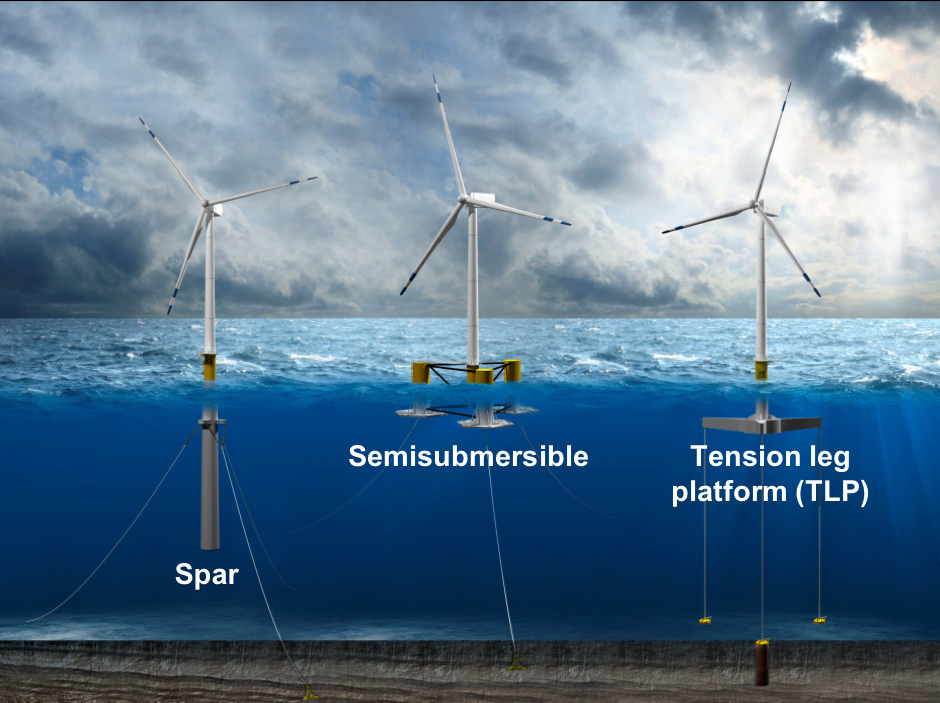
\includegraphics[width=3.75in]{archetypes}
    \caption{Three classical designs for floating turbine substructures.}
    \label{fig:archetype}
  \end{center}
\end{figure}

Similar to \citet{karimi2017}, care was taken to parameterize the
substructure in a general manner, so as to be able to use the same set
of design variables to describe spars, semisubmersibles, TLPs, and
hybrids of those archetypes.  The intent is that this modular approach
to substructure definition will enable rapid analysis of the majority of
designs currently proposed by the floating wind development community,
whether classical or novel in nature.  Furthermore, generalizing the
substructure definition also empowers the optimization algorithm to
search a broad tradespace more efficiently by moving fluidly from one
region to another.

With that intent in mind, the general configuration of a spar-type
substructure is shown in Figure \ref{fig:diagram}, with nomenclature
borrowed from the field of naval architecture.  A semisubmersible
configuration would have a similar diagram, but with multiple offset
columns connected with pontoon elements.  A TLP might look similar to a
spar or semisubmersible, with taut mooring lines instead of the catenary
ones shown.

\begin{figure}[htb]
  \begin{center}
    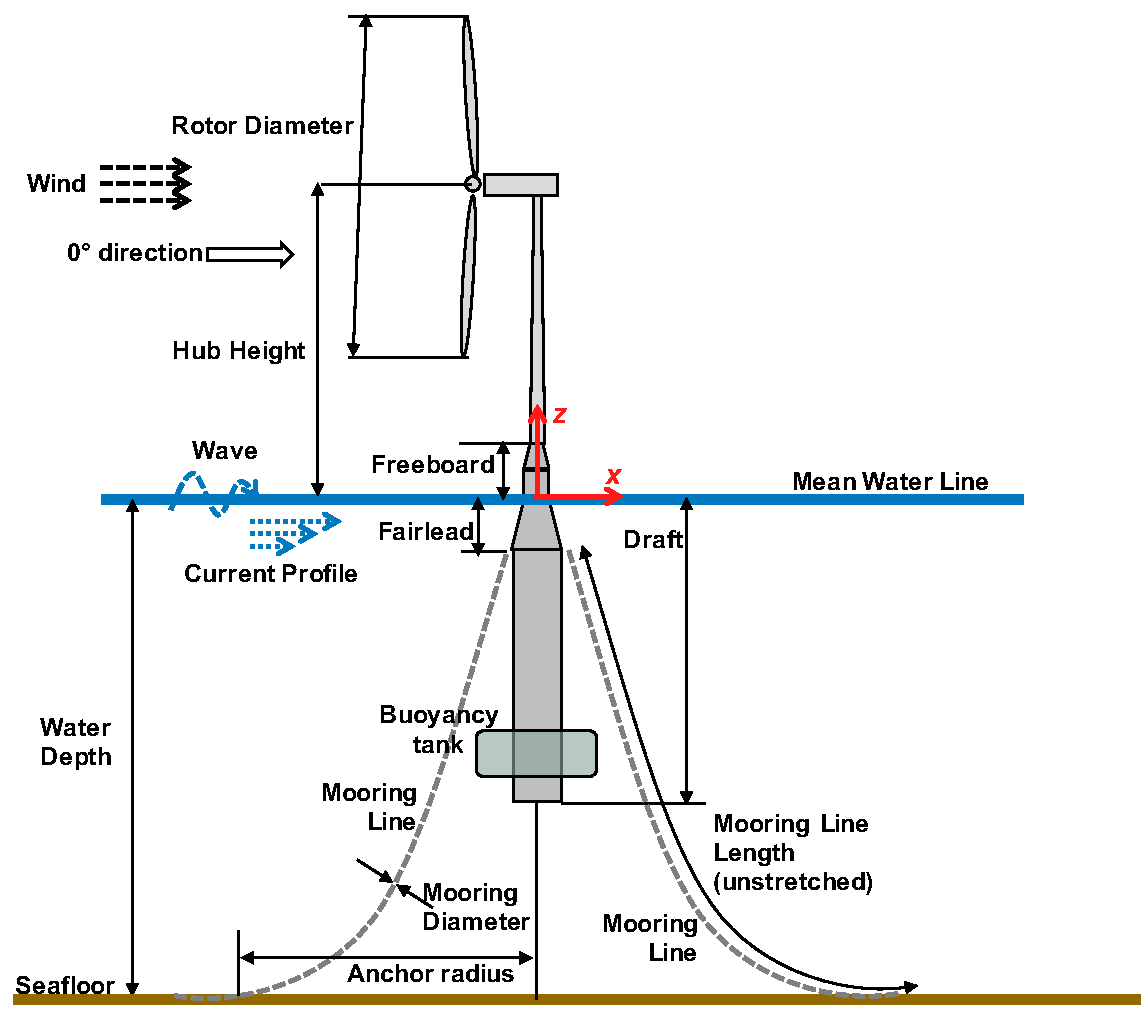
\includegraphics[width=5in]{diagram}
    \caption{Geometry parameterization with common wind turbine and
      naval architecture conventions.}
    \label{fig:diagram}
  \end{center}
\end{figure}

\section{Tapered Cylinders (Vertical Frustums)}
A number of typical floating substructure designs, such as the spar or
semisubmersible, contain vertically oriented columns.  In
\textit{FloatingSE}, these columns are
assumed to have a circular cross-section making them, formally, vertical
frustums.  These frustums are assumed to be ring-stiffened to support
the buckling loads inherent in a submerged support structure.  The
number of columns, their geometry, and the ring stiffeners are
parameterized in the \textit{FloatingSE} module according to the
diagrams in Figures \ref{fig:diagram} and \ref{fig:column}.  The main
column is assumed to centered at $(x=0, y=0)$, directly underneath the
turbine tower (note that off-centered turbines are not yet supported).
Other columns are referred to as \textit{offset} columns, and are
assumed to be evenly spread around the main column.  The material of the
vertical columns is currently assumed to be ASTM 992 steel.
Future developments will include the option to select one of multiple
material options for each section in each cylinder.

\begin{figure}[htb]
  \begin{subfigure}[b]{0.38\linewidth}
    \centering 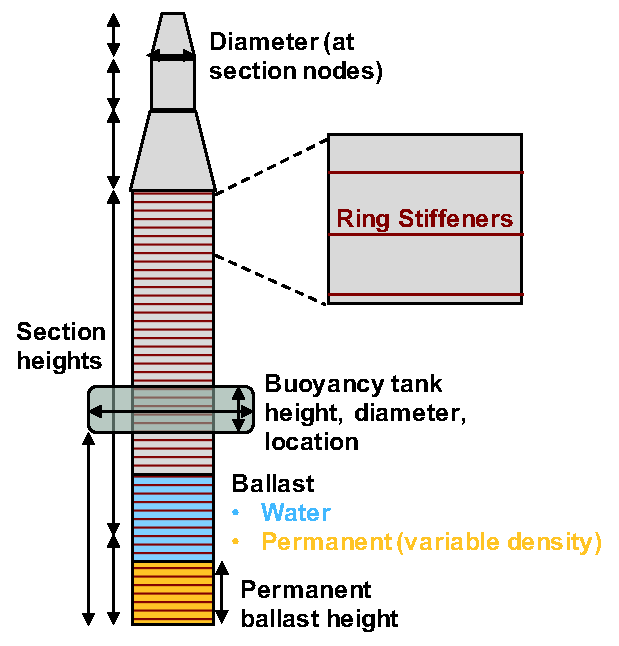
\includegraphics[width=2.2in]{colGeom}
    \caption{Vertical column of frustums}
  \end{subfigure}
  \begin{subfigure}[b]{0.29\linewidth}
    \centering 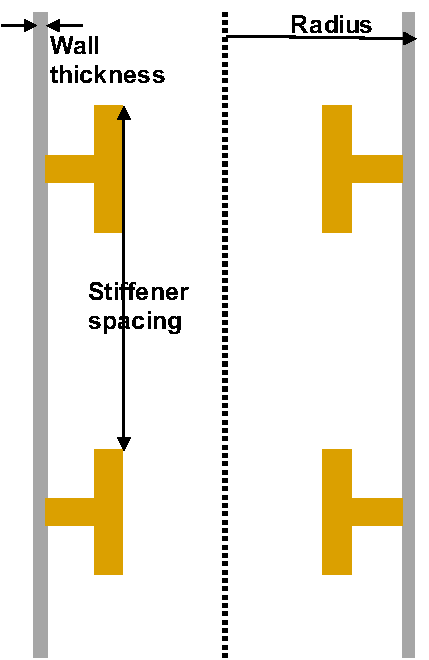
\includegraphics[width=1.8in]{stiffenerCut}
    \caption{Vertical cross-section}
  \end{subfigure}
  \begin{subfigure}[b]{0.29\linewidth}
    \centering 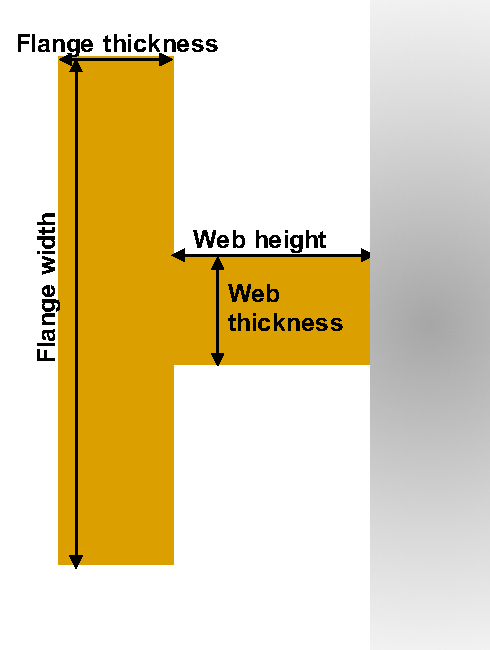
\includegraphics[width=1.8in]{stiffenerZoom}
    \caption{Ring stiffener geometry}
  \end{subfigure}
  \caption{Vertical frustum geometry parameterization.}
  \label{fig:column}
\end{figure}

\section{Discretization}
To allow for varying geometry parameters along the length of
substructure columns, the larger components are divided into sections.
The user may specify the number of overall sections, $n_s$ and the
geometry of each section.  Some of the geometry parameters are tied to
the nodes that bracket each section, such as column diameter and wall
thickness, with linear variation between each node.  Other parameters
are considered constant within each section, such as the spacing between
ring stiffeners.  The number of sections should resemble the physical
number of cans or sections used in the manufacturing of the real
article.

\subsection{Ballast}
Substructure columns with long drafts can enhance stability by placing
heavy ballast, such as magnetite iron ore, at their bottom sections.
The user can specify the density of the permanent ballast added and the
height of the ballast extent within the column.  Variable ballast, as
opposed to permanent ballast, is water that is added or removed above
the permanent ballast to achieve neutral buoyancy as the operating
conditions of the turbine change.  A discussion of variable water
balance in the model is found in Section \ref{sec:static}.

\subsection{Buoyancy Tanks (and Heave Plates)}
Buoyancy tanks are modeled as a collar around the column and are not
subject the same taper or connectivity constraints as the frustum
sections.  They therefore offer added buoyancy without incurring as much
structural mass or cost.  Moreover, they can also serve to augment the
heave added mass like a plate.  In addition to their diameter and
height, the user can adjust the location of the buoyancy tank from the
column base to the top. Buoyancy tanks can be added to either the main
and/or offset columns.

\section{Pontoons and Support Structure}
Many substructure designs include the use of pontoons that form a truss
to connect the different components, usually columns, together.  In this
model, all of the pontoons are assumed to have the identical thin-walled
tube cross section and made of the same material as the rest of the
substructure.  The truss configuration and the parameterization of the
pontoon elements is based on the members shown in Figure
\ref{fig:pontoon} with lettered labels.  The members are broken out into
the upper and lower rings connecting the offset columns ($B$ and $D$,
respectively), the upper and lower main-to-offset connections ($A$ and
$C$, respectively), the lower-base to upper-offset cross members ($E$),
and the V-shaped cross members between offset columns ($F$).

\begin{figure}[htb]
  \begin{center}
    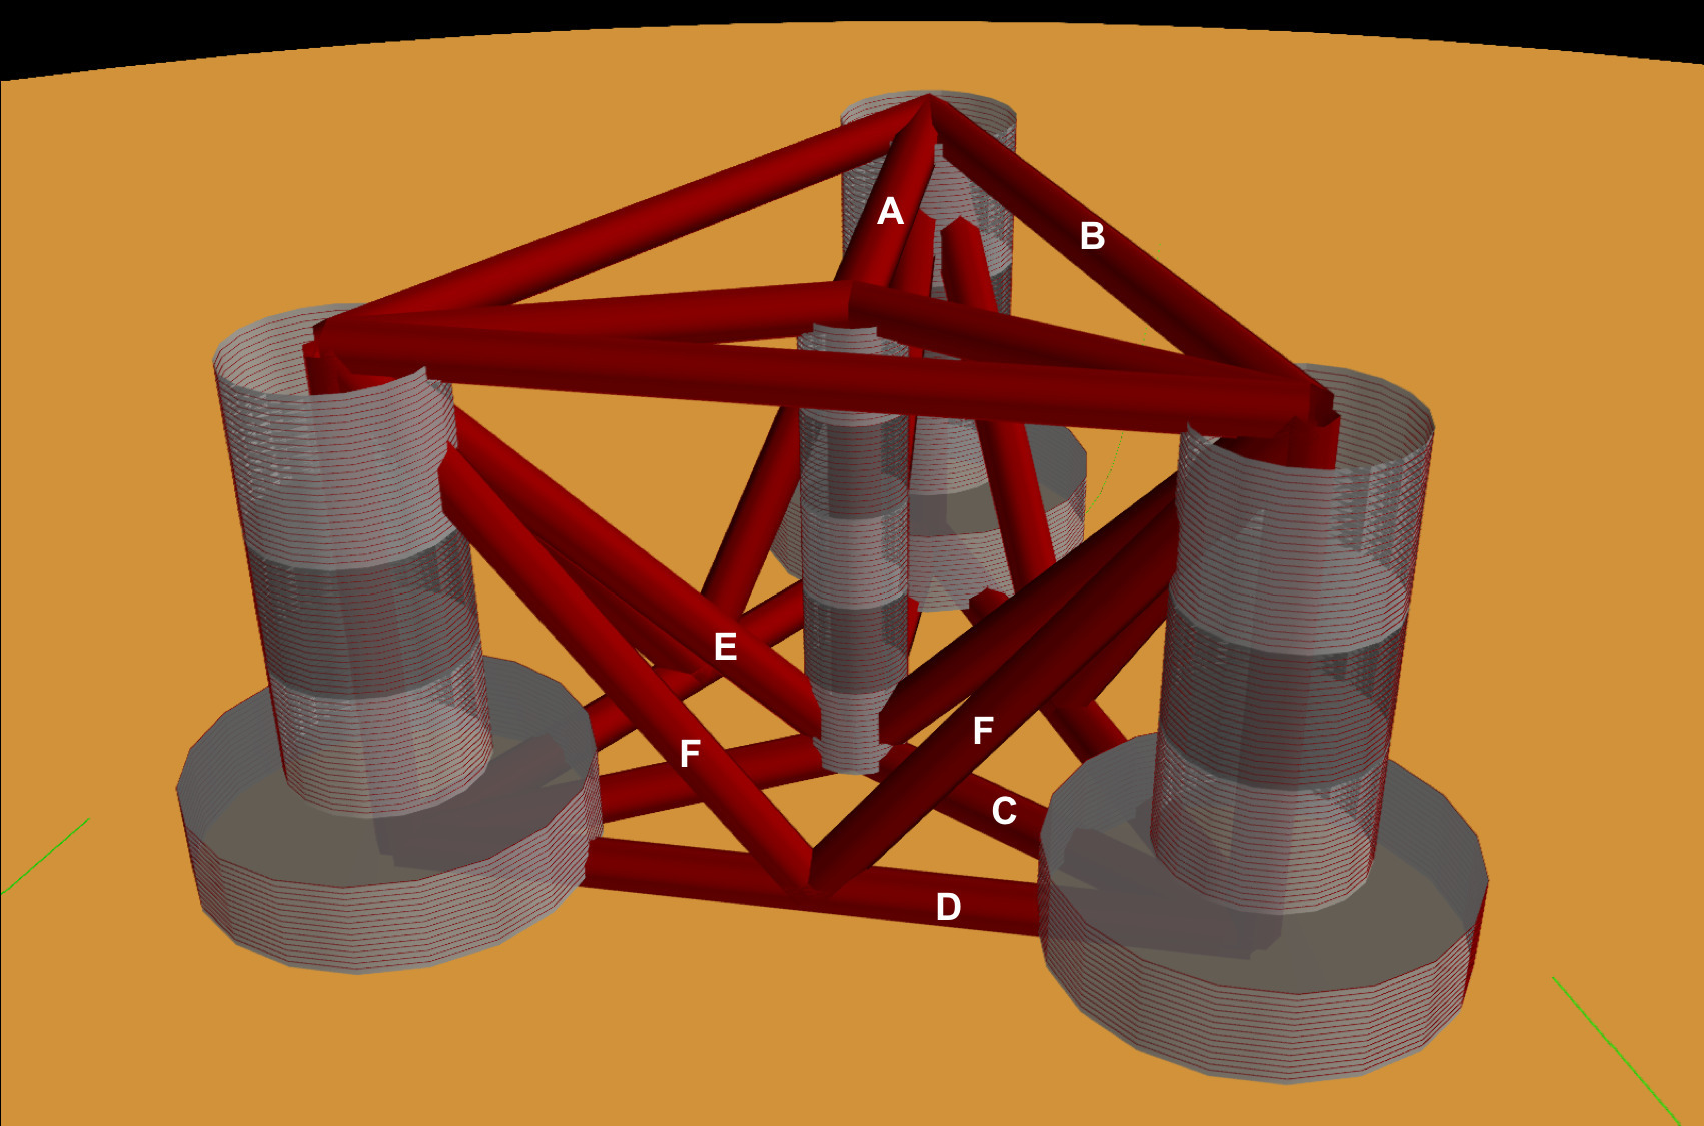
\includegraphics[width=4.5in]{semi}
    \caption{Parameterization of truss elements in substructure.}
    \label{fig:pontoon}
  \end{center}
\end{figure}


\section{Mooring Lines}
The mooring system is described by the number of lines, their geometry,
and their interface to the substructure.  The mooring diameter is set by
the user and determines the breaking load and stiffness of the chain,
via correlation, described in Section \ref{sec:theory}.  The mooring
lines attach to the substructure at the \textit{fairlead} distance below
the water plane, as shown in Figure \ref{fig:diagram}.  The lines can
attach directly to a substructure column or at a some offset from the
outer shell.  Note that bridle connections are not yet implemented.  The
mooring lines attach to the sea floor at a variable distance, the anchor
radius, from the substructure centerline, also set by the user.

By default, the mooring system is assumed to use a steel chain with drag
embedment anchors. Other mooring available for selection are nylon,
polyester, steel wire rope (IWRC) and fiber-core wire rope.  The only
alternative anchor type is currently suction pile anchors, but there are
plans to include gravity anchors as well.  The standard configuration
for TLPs is the use of taut nylon mooring lines with suction-pile
anchors.

\section{Mass and Cost Scaling}
The mass of all components in the modeled substructure is captured
through calculation of each components' volume and multiplying by its material
density.  This applies to the frustum shells, the ring stiffeners, the
permanent ballast, the pontoons, and the mooring lines.
However, the model also acknowledges that the modeled substructure is
merely an approximation of an actual substructure and various secondary
elements are not captured.  These include ladders, walkways, handles,
finishing, paint, wiring, etc.  To account for these features en masse,
multipliers of component masses are offered as parameters for the user
as well.  Capital cost for all substructure components except the
mooring system is assumed to be a linear scaling of the components
masses.  For the mooring system, cost is dependent on the tension
carrying capacity of the line, which itself is an empirical function of
the diameter.  Default values for all mass and cost scaling factors are
found in Table \ref{tbl:factors}.  Cost factors are especially difficult to
estimate given the proprietary nature of commercial cost data, so
cost rates and estimates should be considered notional.

\begin{table}[htbp]
  \begin{center}
    {\small
      \caption{Default mass scaling factors and cost rates used in
        \textit{FloatingSE} (notional).}
      \label{tbl:factors}
      \begin{tabular}{llcll}
        \textbf{Mass factor} & \textbf{Value} && \textbf{Cost rate} & \textbf{Value} \\
        \hline \hline
        Bulkhead, stiffener & 1.0 && Ballast & \unit[100]{USD/kg} \\
        Column outfitting & 1.06 && Column outfitting & \unit[6,980]{USD/kg} \\
        Tapered column & 1.05 & Tapered column & \unit[4,720]{USD/kg} \\
        Tower outfitting & 1.07 && Pontoons & \unit[6.5]{USD/kg} \\
        \hline
      \end{tabular}
    }
  \end{center}
\end{table}
